\documentclass[]{article}
\usepackage{lmodern}
\usepackage{amssymb,amsmath}
\usepackage{ifxetex,ifluatex}
\usepackage{fixltx2e} % provides \textsubscript
\ifnum 0\ifxetex 1\fi\ifluatex 1\fi=0 % if pdftex
  \usepackage[T1]{fontenc}
  \usepackage[utf8]{inputenc}
\else % if luatex or xelatex
  \ifxetex
    \usepackage{mathspec}
  \else
    \usepackage{fontspec}
  \fi
  \defaultfontfeatures{Ligatures=TeX,Scale=MatchLowercase}
  \newcommand{\euro}{€}
\fi
% use upquote if available, for straight quotes in verbatim environments
\IfFileExists{upquote.sty}{\usepackage{upquote}}{}
% use microtype if available
\IfFileExists{microtype.sty}{%
\usepackage{microtype}
\UseMicrotypeSet[protrusion]{basicmath} % disable protrusion for tt fonts
}{}
\usepackage[margin=1in]{geometry}
\usepackage{hyperref}
\PassOptionsToPackage{usenames,dvipsnames}{color} % color is loaded by hyperref
\hypersetup{unicode=true,
            pdftitle={Building Energy Simulation Paper Title},
            pdfauthor={H. Berk, D. Fanelli J. Hamski, S. Hong},
            pdfborder={0 0 0},
            breaklinks=true}
\urlstyle{same}  % don't use monospace font for urls
\usepackage{longtable,booktabs}
\usepackage{graphicx,grffile}
\makeatletter
\def\maxwidth{\ifdim\Gin@nat@width>\linewidth\linewidth\else\Gin@nat@width\fi}
\def\maxheight{\ifdim\Gin@nat@height>\textheight\textheight\else\Gin@nat@height\fi}
\makeatother
% Scale images if necessary, so that they will not overflow the page
% margins by default, and it is still possible to overwrite the defaults
% using explicit options in \includegraphics[width, height, ...]{}
\setkeys{Gin}{width=\maxwidth,height=\maxheight,keepaspectratio}
\setlength{\parindent}{0pt}
\setlength{\parskip}{6pt plus 2pt minus 1pt}
\setlength{\emergencystretch}{3em}  % prevent overfull lines
\providecommand{\tightlist}{%
  \setlength{\itemsep}{0pt}\setlength{\parskip}{0pt}}
\setcounter{secnumdepth}{5}

%%% Use protect on footnotes to avoid problems with footnotes in titles
\let\rmarkdownfootnote\footnote%
\def\footnote{\protect\rmarkdownfootnote}

%%% Change title format to be more compact
\usepackage{titling}

% Create subtitle command for use in maketitle
\newcommand{\subtitle}[1]{
  \posttitle{
    \begin{center}\large#1\end{center}
    }
}

\setlength{\droptitle}{-2em}
  \title{Building Energy Simulation Paper Title}
  \pretitle{\vspace{\droptitle}\centering\huge}
  \posttitle{\par}
  \author{H. Berk, D. Fanelli J. Hamski, S. Hong}
  \preauthor{\centering\large\emph}
  \postauthor{\par}
  \predate{\centering\large\emph}
  \postdate{\par}
  \date{11/27/2016}


% Redefines (sub)paragraphs to behave more like sections
\ifx\paragraph\undefined\else
\let\oldparagraph\paragraph
\renewcommand{\paragraph}[1]{\oldparagraph{#1}\mbox{}}
\fi
\ifx\subparagraph\undefined\else
\let\oldsubparagraph\subparagraph
\renewcommand{\subparagraph}[1]{\oldsubparagraph{#1}\mbox{}}
\fi


\begin{document}
\maketitle

\section{Abstract}\label{abstract}

\section{Introduction}\label{introduction}

The U.S Energy Information Administration's Commercial Buildings Energy
Consumption Survey (CBECS) estimates that there were 5.6 million
commercial buildings in the United States in 2012, comprising 87 billion
square feet of floorspace. These buildings consumed 6,963 trillion Btu
in site energy. In 2014, New York City buildings were responsible for 73
percent of citywide greenhouse gas (GHG) emissions through the use of
natural gas, electricity, heating oil, steam, and biofuel.

We propose to build on the methodology described in the papers below on
change-point regression modeling of building energy use to investigate
energy use in New York City. The practice of using inverse modeling to
analyze historical facility energy consumption has been widely
researched and employed in the industry since the late 1990s; however,
the proposed inverse simulation methodology is a relatively new concept
and has not been widely reviewed in the literature. As the research in
question was developed on industrial facilities and single-family homes,
it is unclear as to whether the methodology is applicable to the
commercial real estate sector (i.e., office buildings) in New York City.

\section{Literature Review}\label{literature-review}

\section{Methodology}\label{methodology}

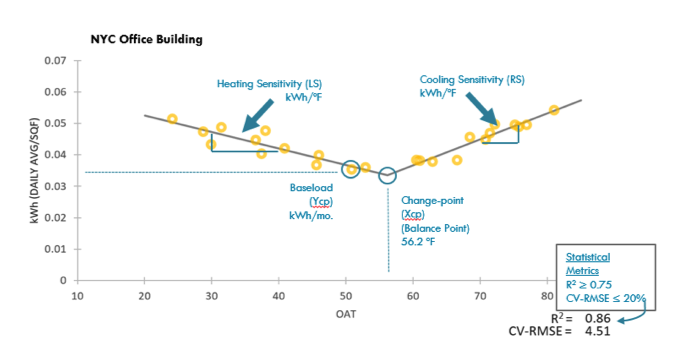
\includegraphics{NYCOfficeBuilding.png}

\subsection{Data Sources \& Preparation}\label{data-sources-preparation}

\subsection{Building Comparison
(Sonya)}\label{building-comparison-sonya}

\subsection{Change-point Regression}\label{change-point-regression}

Heating and cooling energy consumption varies according to ambient air
temperature in addition to baseline use for non-temperature regulating
consumtion like cooking (gas) or lighting (electricity). A changepoint
analysis was preformed on both electricty and fuel data using the R
package \emph{changepoint} (Killick and Eckley, 2014).

The changepoint analysis utilized the AMOC method (At Most One Change)
to specify a single changepoint for each electricity and fuel
consumption series with no loss function. For electricty, the
changepoint was determined using the mean of the electricty load data.
Given the wide range of electricity loads over the observed temperature
range, the change in mean at warmer temperatures leads to an
identifiable changepoint. For fuel, both mean and variance changes were
incorporated to determine the changepoint, as at warmer temperatures
there is very little change in the fuel load (i.e.~the baseline load has
very little variance, but the load during warming temperatures does).

After determining the changepoints, a linear regression model was fit to
the electricty load observations at temperatures greater than or equal
to the changepoint. For fuel load the linear regression model was fit to
observations less than or equal to the changepoint. These two linear
models represent the observed response rates of energy load to changes
in average monthly outside air temperature.

\begin{longtable}[c]{@{}llllll@{}}
\toprule
& EXC & LIC & MFC & MSC & SUN\tabularnewline
\midrule
\endhead
Elec & 47600 & 25200 & 430400 & 215323 & 257600\tabularnewline
AveTemp & 62.75806 & 62.75806 & 66.13548 & 66.13548 &
66.13548\tabularnewline
\bottomrule
\end{longtable}

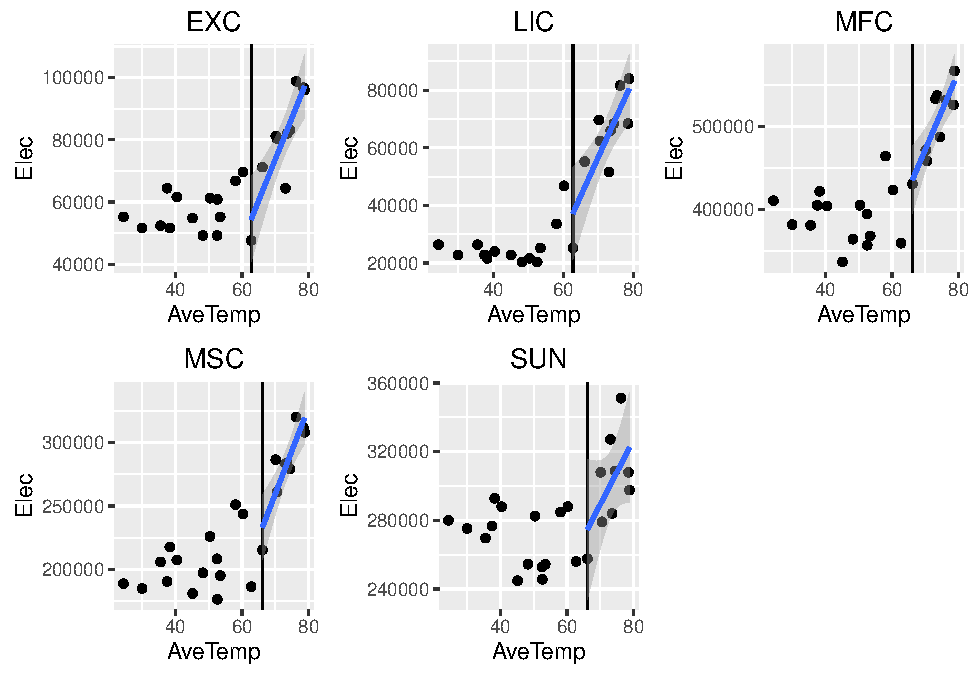
\includegraphics{Paper-BuildingEnergySim_files/figure-latex/unnamed-chunk-2-1.pdf}

\begin{longtable}[c]{@{}llllll@{}}
\toprule
& EXC & LIC & MFC & MSC & SUN\tabularnewline
\midrule
\endhead
Fuel & 876396000 & 185900000 & 992214000 & 578397958 &
4776000\tabularnewline
AveTemp & 62.75806 & 66.13548 & 52.57667 & 58.06452 &
70.53\tabularnewline
\bottomrule
\end{longtable}

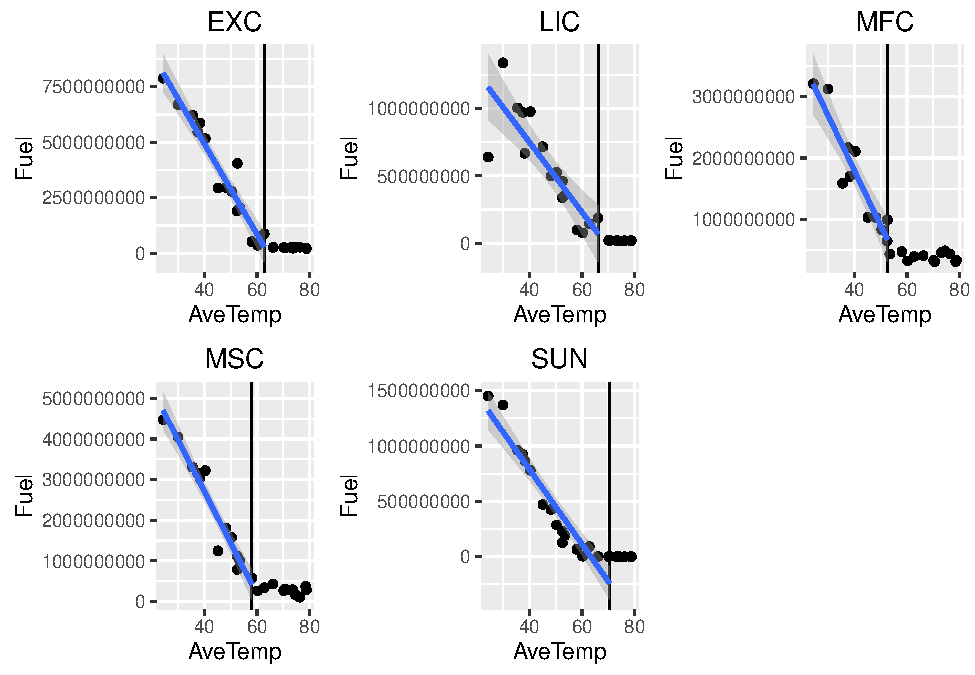
\includegraphics{Paper-BuildingEnergySim_files/figure-latex/unnamed-chunk-3-1.pdf}

\begin{verbatim}
## 
## Call:
## lm(formula = Elec ~ AveTemp, data = df %>% filter(Facility == 
##     bldg) %>% filter(AveTemp >= elec.changepoints["AveTemp", 
##     ]$bldg))
## 
## Coefficients:
## (Intercept)      AveTemp  
##     -131947         2695
\end{verbatim}

\begin{verbatim}
##              LIC
## AveTemp 62.75806
##        LIC
## Elec 25200
\end{verbatim}

\begin{verbatim}
##        1 
## 83687.98
\end{verbatim}

\subsubsection{Building:LIC Model}\label{buildinglic-model}

\begin{verbatim}
## Expected kWh at Toa: 0.04471509
\end{verbatim}

\begin{verbatim}
## Cooling Coefficient: 15502.5
\end{verbatim}

\begin{verbatim}
## Cooling efficiency: 13383842
\end{verbatim}

\begin{verbatim}
## Internal loads: 178588.9
\end{verbatim}

\begin{verbatim}
##           parameters
## 1         0.31000000
## 2     50000.00000000
## 3         2.00000000
## 4         1.19600000
## 5         1.04700000
## 6         0.00115830
## 7        53.48000000
## 8        65.00000000
## 9         0.01399697
## 10       80.00000000
## 11        0.04471509
## 12    15502.50442400
## 13 13383842.20322887
## 14   178588.85096448
\end{verbatim}

\begin{verbatim}
##              U              A              V            rho             cp 
##        0.31000    50000.00000        2.00000        1.19600        1.04700 
##             CS           TcpC           Tset             Ei            Toa 
##        0.00116       53.48000       65.00000        0.01400       80.00000 
##              E             CC           Effc             Qi 
##        0.04472    15502.50442 13383842.20323   178588.85096
\end{verbatim}

\begin{verbatim}
## Expected kWh at Toa: 0.04471509
\end{verbatim}

\begin{verbatim}
## Cooling Coefficient: 15502.5
\end{verbatim}

\begin{verbatim}
## Cooling efficiency: 13383842
\end{verbatim}

\begin{verbatim}
## Internal loads: 178588.9
\end{verbatim}

\emph{Assumptions made for model can be simulated:}\\
- Sim \#1: Toa -- use CP Model Equation and simulate Toa from 10-100
degrees F in steps of 5 degrees\\
- Sim \#2: Tset -- substitute other values from 50 to 75, in steps of 5
degrees -- this simulates setting the thermostat lower or higher\\
- Sim \#3: U -- substitute other values: 0.25, 0.18, 0.12, 0.09 -- this
simulates adding insulation, etc. to tighten building envelope\\
- Sim \#4: V -- substitute other values: 1 to 3, in steps of 0.5 -- this
simulates improved/worse ventilation/infiltration flow rate (lower is)

\section{Sim 1: Toa}\label{sim-1-toa}

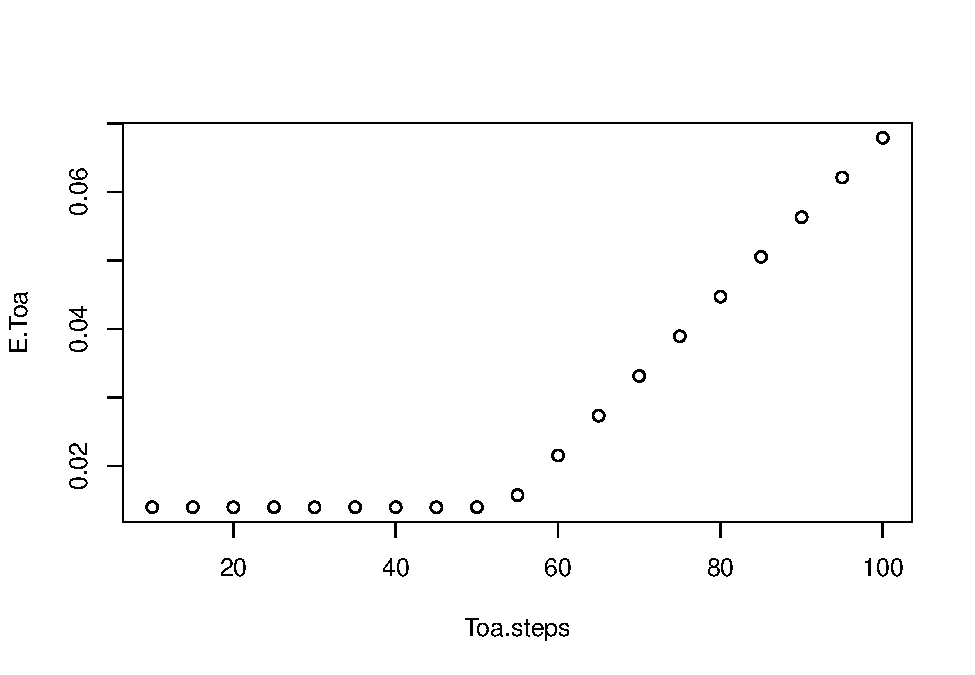
\includegraphics{Paper-BuildingEnergySim_files/figure-latex/unnamed-chunk-9-1.pdf}

\subsubsection{Weather Sampling
Utilities:}\label{weather-sampling-utilities}

We need a single temperature per month, but that single temperature can
be chosen in a variety of ways. Various strategies could include the
following:

\begin{itemize}
\tightlist
\item
  The mean temperature for the specified month and year
\item
  The maximum temperature for the specified month and year
\item
  The minimum temperature for the specified month and year
\item
  The maximum temperature for the specified month for ALL years
\end{itemize}

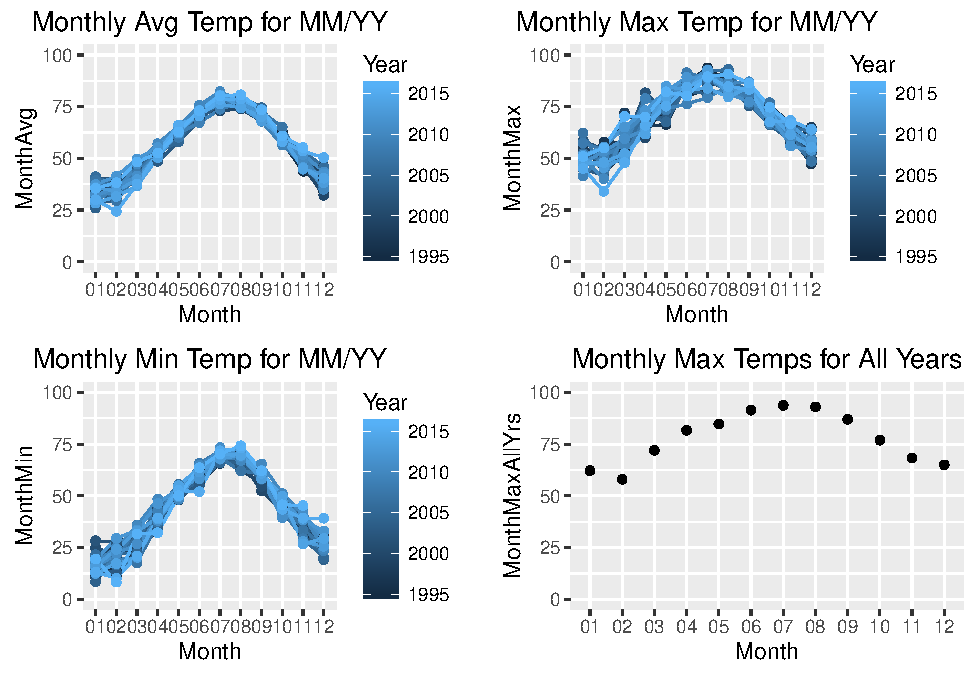
\includegraphics{Paper-BuildingEnergySim_files/figure-latex/unnamed-chunk-10-1.pdf}

\subsubsection{Random Sampled Temperatures by
Month}\label{random-sampled-temperatures-by-month}

We will sample a random day per month for the specified year as our
sampling strategy. Below is an example of the output:

\begin{verbatim}
##    [1995 Month] [1995 Sampled Temps]
## 1            01                 56.9
## 2            02                 31.3
## 3            03                 47.6
## 4            04                 52.2
## 5            05                 50.7
## 6            06                 76.8
## 7            07                 81.2
## 8            08                 73.2
## 9            09                 68.3
## 10           10                 61.7
## 11           11                 46.3
## 12           12                 41.5
\end{verbatim}

\begin{verbatim}
##    [1997 Month] [1997 Sampled Temps]
## 1            01                 36.4
## 2            02                     
## 3            03                 37.5
## 4            04                 51.4
## 5            05                 57.3
## 6            06                 55.8
## 7            07                   76
## 8            08                 74.7
## 9            09                 75.1
## 10           10                 72.6
## 11           11                 35.2
## 12           12                 47.2
\end{verbatim}

\begin{verbatim}
##    [1999 Month] [1999 Sampled Temps]
## 1            01                 25.5
## 2            02                   36
## 3            03                 43.4
## 4            04                   53
## 5            05                 60.8
## 6            06                 78.8
## 7            07                 83.1
## 8            08                   65
## 9            09                 65.9
## 10           10                 50.9
## 11           11                 59.9
## 12           12                 30.2
\end{verbatim}

\subsection{Sensitivity Analysis and Temperature
Sampling}\label{sensitivity-analysis-and-temperature-sampling}

\section{Results}\label{results}

\section{Conclusions}\label{conclusions}

\section{Citations}\label{citations}

Killick, R., Eckley, I., changepoint: An R Package for Changepoint
Analysis. Journal of Statistical Software, June 2014 58:3.

\section{Appendix I - Figures \&
Tables}\label{appendix-i---figures-tables}

\end{document}
